\documentclass[11pt]{article}
\def\activityid{F01-X / FACILITATOR}% Week 1 v2. Shared style and exact unit-edge geometry.
\usepackage[letterpaper,margin=.65in,top=.60in,bottom=.65in]{geometry}
\usepackage[T1]{fontenc}
\usepackage[default]{sourcesanspro}
\usepackage{microtype,tikz,array,tabularx,fancyhdr,amsmath}
\usepackage[hidelinks]{hyperref}
\usetikzlibrary{calc,arrows.meta}
\setlength{\parindent}{0pt}\setlength{\parskip}{7pt}
\setlength{\headheight}{0pt}\setlength{\footskip}{26pt}
\setlength{\emergencystretch}{2em}
\pagestyle{fancy}\fancyhf{}\renewcommand{\headrulewidth}{0pt}\renewcommand{\footrulewidth}{.4pt}
\fancyfoot[L]{\scriptsize Bellingham Math Circle / Week 1 / \activityid}
\fancyfoot[R]{\scriptsize \thepage}
\definecolor{ink}{gray}{.12}\definecolor{soft}{gray}{.95}\color{ink}
\newlength{\blockside}\setlength{\blockside}{1in}
\def\hh{0.8660254037844386}
\tikzset{outline/.style={draw=ink,line width=1.05pt,line join=round},tile/.style={draw=ink,line width=.65pt,line join=round},gridline/.style={draw=black!40,line width=.35pt}}
\newcommand{\HexPath}{(-1,0)--(-.5,-\hh)--(.5,-\hh)--(1,0)--(.5,\hh)--(-.5,\hh)--cycle}
\newcommand{\BluePath}{(0,0)--(1,0)--(1.5,\hh)--(.5,\hh)--cycle}
\newcommand{\ChevronPath}{(0,0)--(1,0)--(1.5,\hh)--(1,2*\hh)--(0,2*\hh)--(.5,\hh)--cycle}
\newcommand{\BoardPath}{(0,0)--(1,0)--(2,2*\hh)--(1,4*\hh)--(0,4*\hh)--(-1,2*\hh)--cycle}
\newcommand{\PageTitle}[2]{{\fontsize{10}{12}\selectfont\bfseries WEEK 1\quad TILING LAB\hfill #1\par}\vspace{3pt}{\fontsize{27}{30}\selectfont\bfseries #2\par}\vspace{2pt}}
\newcommand{\NameLine}{{\small Name: \rule{2.65in}{.4pt}\hfill Date: \rule{1.35in}{.4pt}\par}\vspace{4pt}}
\newcommand{\Task}[2]{\par\vspace{3pt}{\large\bfseries #1}\par #2\par}
\newcommand{\Subhead}[1]{\par\vspace{3pt}{\large\bfseries #1}\par}
\newcommand{\RuleBox}[1]{\par\begingroup\setlength{\fboxsep}{8pt}\colorbox{soft}{\parbox{\dimexpr\linewidth-16pt\relax}{#1}}\endgroup\par}
\newcommand{\WriteBox}[2]{\par\textbf{#1}\par\vspace{2pt}\begin{tikzpicture}\draw[black!40,line width=.5pt] (0,0) rectangle (\dimexpr\linewidth-.5pt\relax,#2);\end{tikzpicture}\par}
\newcommand{\DrawOutline}[1]{\begin{tikzpicture}[x=\blockside,y=\blockside]\draw[outline] #1;\end{tikzpicture}}
\newcommand{\Pair}[1]{\par\vspace{4pt}\begin{minipage}[t]{.485\linewidth}\centering\textbf{First filling}\par\vspace{8pt}\DrawOutline{#1}\end{minipage}\hfill\begin{minipage}[t]{.485\linewidth}\centering\textbf{Another filling}\par\vspace{8pt}\DrawOutline{#1}\end{minipage}\par}
\newcommand{\ScaleCheck}{\vfill\par\begingroup\fontsize{9}{11}\selectfont\begin{minipage}[c]{1.2in}\centering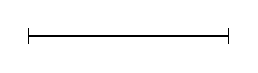
\begin{tikzpicture}[x=\blockside,y=1in]\draw[line width=.65pt] (0,0)--(1,0);\draw (0,-.04)--(0,.04) (1,-.04)--(1,.04);\end{tikzpicture}\par One small block edge\end{minipage}\hfill\begin{minipage}[c]{\dimexpr\linewidth-1.35in\relax}Adult: print \textbf{100\% / Actual Size}, single-sided. Default edge: 1 inch (25.4 mm). Compare with a \textbf{1\(\times\)} green triangle before using these mats.\end{minipage}\par\endgroup}
\newcommand{\StudentFooter}{\vfill{\small Build first. Explain by pointing, talking, or drawing.}\par}
\newcommand{\UnitRule}{Use the small (1\(\times\)) pieces. Turn them as needed.}
% An upward side-n triangle, with unit cells and no solution lines.
\newcommand{\TriangleGrid}[1]{
 \pgfmathtruncatemacro{\nn}{#1-1}
 \foreach \j in {0,...,\nn}{\pgfmathtruncatemacro{\imax}{#1-1-\j}\foreach \i in {0,...,\imax}{\draw[gridline] ({\i+.5*\j},{\hh*\j})--({\i+1+.5*\j},{\hh*\j})--({\i+.5*\j+.5},{\hh*(\j+1)})--cycle;}}
 \draw[outline] (0,0)--(#1,0)--({#1/2},{#1*\hh})--cycle;}
\newcommand{\TriangleMat}[1]{\begin{tikzpicture}[x=\blockside,y=\blockside]\TriangleGrid{#1}\end{tikzpicture}}
\newcommand{\HexBlues}{\draw[tile] \HexPath;\draw[tile] (0,0)--(1,0) (0,0)--(-.5,\hh) (0,0)--(-.5,-\hh);}
\newcommand{\FlipExample}{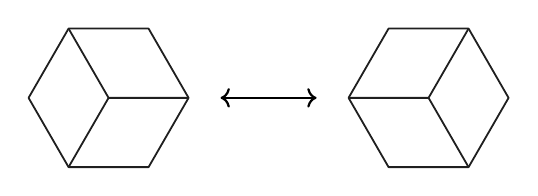
\begin{tikzpicture}[x=.40in,y=.40in]\HexBlues\begin{scope}[shift={(4,0)},rotate=60]\HexBlues\end{scope}\draw[<->,thick] (1.4,0)--(2.6,0);\end{tikzpicture}}
\newcommand{\StatePic}[2]{\begin{tikzpicture}[x=#2\blockside,y=#2\blockside]\csname Tiling#1\endcsname\draw[outline] \BoardPath;\draw[line width=2pt] (0,0)--(1,0);\end{tikzpicture}}
\newcommand{\StateCard}[1]{\begin{minipage}[t]{.30\linewidth}\centering\textbf{#1}\par\StatePic{#1}{.32}\end{minipage}}
% Generated by generate-geometry.py; coordinate unit = one small block edge.
\newcommand{\BoardGrid}{\draw[gridline] (-0.500000000,0.866025404)--(0.000000000,1.732050808)--(-1.000000000,1.732050808)--cycle;\draw[gridline] (-1.000000000,1.732050808)--(0.000000000,1.732050808)--(-0.500000000,2.598076211)--cycle;\draw[gridline] (0.000000000,1.732050808)--(0.500000000,2.598076211)--(-0.500000000,2.598076211)--cycle;\draw[gridline] (-0.500000000,2.598076211)--(0.500000000,2.598076211)--(0.000000000,3.464101615)--cycle;\draw[gridline] (0.500000000,2.598076211)--(1.000000000,3.464101615)--(0.000000000,3.464101615)--cycle;\draw[gridline] (0.000000000,0.000000000)--(0.500000000,0.866025404)--(-0.500000000,0.866025404)--cycle;\draw[gridline] (-0.500000000,0.866025404)--(0.500000000,0.866025404)--(0.000000000,1.732050808)--cycle;\draw[gridline] (0.500000000,0.866025404)--(1.000000000,1.732050808)--(0.000000000,1.732050808)--cycle;\draw[gridline] (0.000000000,1.732050808)--(1.000000000,1.732050808)--(0.500000000,2.598076211)--cycle;\draw[gridline] (1.000000000,1.732050808)--(1.500000000,2.598076211)--(0.500000000,2.598076211)--cycle;\draw[gridline] (0.500000000,2.598076211)--(1.500000000,2.598076211)--(1.000000000,3.464101615)--cycle;\draw[gridline] (0.000000000,0.000000000)--(1.000000000,0.000000000)--(0.500000000,0.866025404)--cycle;\draw[gridline] (1.000000000,0.000000000)--(1.500000000,0.866025404)--(0.500000000,0.866025404)--cycle;\draw[gridline] (0.500000000,0.866025404)--(1.500000000,0.866025404)--(1.000000000,1.732050808)--cycle;\draw[gridline] (1.500000000,0.866025404)--(2.000000000,1.732050808)--(1.000000000,1.732050808)--cycle;\draw[gridline] (1.000000000,1.732050808)--(2.000000000,1.732050808)--(1.500000000,2.598076211)--cycle;}
\newcommand{\TilingA}{\draw[tile] (-0.500000000,0.866025404)--(0.000000000,1.732050808)--(-0.500000000,2.598076211)--(-1.000000000,1.732050808)--cycle;\draw[tile] (0.000000000,1.732050808)--(0.500000000,2.598076211)--(0.000000000,3.464101615)--(-0.500000000,2.598076211)--cycle;\draw[tile] (0.500000000,2.598076211)--(1.500000000,2.598076211)--(1.000000000,3.464101615)--(0.000000000,3.464101615)--cycle;\draw[tile] (0.000000000,0.000000000)--(0.500000000,0.866025404)--(0.000000000,1.732050808)--(-0.500000000,0.866025404)--cycle;\draw[tile] (0.500000000,0.866025404)--(1.000000000,1.732050808)--(0.500000000,2.598076211)--(0.000000000,1.732050808)--cycle;\draw[tile] (1.000000000,1.732050808)--(2.000000000,1.732050808)--(1.500000000,2.598076211)--(0.500000000,2.598076211)--cycle;\draw[tile] (0.000000000,0.000000000)--(1.000000000,0.000000000)--(1.500000000,0.866025404)--(0.500000000,0.866025404)--cycle;\draw[tile] (0.500000000,0.866025404)--(1.500000000,0.866025404)--(2.000000000,1.732050808)--(1.000000000,1.732050808)--cycle;}
\newcommand{\PathA}{\draw[-{Stealth[length=4pt]},line width=1.2pt,dashed] (0.500000000,0.000000000)--(1.000000000,0.866025404);\draw[-{Stealth[length=4pt]},line width=1.2pt,dashed] (1.000000000,0.866025404)--(1.500000000,1.732050808);\draw[-{Stealth[length=4pt]},line width=1.2pt,dashed] (1.500000000,1.732050808)--(1.000000000,2.598076211);\draw[-{Stealth[length=4pt]},line width=1.2pt,dashed] (1.000000000,2.598076211)--(0.500000000,3.464101615);}
\newcommand{\TilingB}{\draw[tile] (-0.500000000,0.866025404)--(0.000000000,1.732050808)--(-0.500000000,2.598076211)--(-1.000000000,1.732050808)--cycle;\draw[tile] (0.000000000,1.732050808)--(0.500000000,2.598076211)--(0.000000000,3.464101615)--(-0.500000000,2.598076211)--cycle;\draw[tile] (0.500000000,2.598076211)--(1.500000000,2.598076211)--(1.000000000,3.464101615)--(0.000000000,3.464101615)--cycle;\draw[tile] (0.000000000,0.000000000)--(0.500000000,0.866025404)--(0.000000000,1.732050808)--(-0.500000000,0.866025404)--cycle;\draw[tile] (0.500000000,0.866025404)--(1.500000000,0.866025404)--(1.000000000,1.732050808)--(0.000000000,1.732050808)--cycle;\draw[tile] (0.000000000,1.732050808)--(1.000000000,1.732050808)--(1.500000000,2.598076211)--(0.500000000,2.598076211)--cycle;\draw[tile] (0.000000000,0.000000000)--(1.000000000,0.000000000)--(1.500000000,0.866025404)--(0.500000000,0.866025404)--cycle;\draw[tile] (1.500000000,0.866025404)--(2.000000000,1.732050808)--(1.500000000,2.598076211)--(1.000000000,1.732050808)--cycle;}
\newcommand{\PathB}{\draw[-{Stealth[length=4pt]},line width=1.2pt,dashed] (0.500000000,0.000000000)--(1.000000000,0.866025404);\draw[-{Stealth[length=4pt]},line width=1.2pt,dashed] (1.000000000,0.866025404)--(0.500000000,1.732050808);\draw[-{Stealth[length=4pt]},line width=1.2pt,dashed] (0.500000000,1.732050808)--(1.000000000,2.598076211);\draw[-{Stealth[length=4pt]},line width=1.2pt,dashed] (1.000000000,2.598076211)--(0.500000000,3.464101615);}
\newcommand{\TilingC}{\draw[tile] (-0.500000000,0.866025404)--(0.000000000,1.732050808)--(-0.500000000,2.598076211)--(-1.000000000,1.732050808)--cycle;\draw[tile] (0.000000000,1.732050808)--(0.500000000,2.598076211)--(0.000000000,3.464101615)--(-0.500000000,2.598076211)--cycle;\draw[tile] (0.500000000,2.598076211)--(1.500000000,2.598076211)--(1.000000000,3.464101615)--(0.000000000,3.464101615)--cycle;\draw[tile] (0.000000000,0.000000000)--(1.000000000,0.000000000)--(0.500000000,0.866025404)--(-0.500000000,0.866025404)--cycle;\draw[tile] (-0.500000000,0.866025404)--(0.500000000,0.866025404)--(1.000000000,1.732050808)--(0.000000000,1.732050808)--cycle;\draw[tile] (0.000000000,1.732050808)--(1.000000000,1.732050808)--(1.500000000,2.598076211)--(0.500000000,2.598076211)--cycle;\draw[tile] (1.000000000,0.000000000)--(1.500000000,0.866025404)--(1.000000000,1.732050808)--(0.500000000,0.866025404)--cycle;\draw[tile] (1.500000000,0.866025404)--(2.000000000,1.732050808)--(1.500000000,2.598076211)--(1.000000000,1.732050808)--cycle;}
\newcommand{\PathC}{\draw[-{Stealth[length=4pt]},line width=1.2pt,dashed] (0.500000000,0.000000000)--(0.000000000,0.866025404);\draw[-{Stealth[length=4pt]},line width=1.2pt,dashed] (0.000000000,0.866025404)--(0.500000000,1.732050808);\draw[-{Stealth[length=4pt]},line width=1.2pt,dashed] (0.500000000,1.732050808)--(1.000000000,2.598076211);\draw[-{Stealth[length=4pt]},line width=1.2pt,dashed] (1.000000000,2.598076211)--(0.500000000,3.464101615);}
\newcommand{\TilingD}{\draw[tile] (-0.500000000,0.866025404)--(0.000000000,1.732050808)--(-0.500000000,2.598076211)--(-1.000000000,1.732050808)--cycle;\draw[tile] (0.000000000,1.732050808)--(1.000000000,1.732050808)--(0.500000000,2.598076211)--(-0.500000000,2.598076211)--cycle;\draw[tile] (-0.500000000,2.598076211)--(0.500000000,2.598076211)--(1.000000000,3.464101615)--(0.000000000,3.464101615)--cycle;\draw[tile] (0.000000000,0.000000000)--(0.500000000,0.866025404)--(0.000000000,1.732050808)--(-0.500000000,0.866025404)--cycle;\draw[tile] (0.500000000,0.866025404)--(1.500000000,0.866025404)--(1.000000000,1.732050808)--(0.000000000,1.732050808)--cycle;\draw[tile] (1.000000000,1.732050808)--(1.500000000,2.598076211)--(1.000000000,3.464101615)--(0.500000000,2.598076211)--cycle;\draw[tile] (0.000000000,0.000000000)--(1.000000000,0.000000000)--(1.500000000,0.866025404)--(0.500000000,0.866025404)--cycle;\draw[tile] (1.500000000,0.866025404)--(2.000000000,1.732050808)--(1.500000000,2.598076211)--(1.000000000,1.732050808)--cycle;}
\newcommand{\PathD}{\draw[-{Stealth[length=4pt]},line width=1.2pt,dashed] (0.500000000,0.000000000)--(1.000000000,0.866025404);\draw[-{Stealth[length=4pt]},line width=1.2pt,dashed] (1.000000000,0.866025404)--(0.500000000,1.732050808);\draw[-{Stealth[length=4pt]},line width=1.2pt,dashed] (0.500000000,1.732050808)--(0.000000000,2.598076211);\draw[-{Stealth[length=4pt]},line width=1.2pt,dashed] (0.000000000,2.598076211)--(0.500000000,3.464101615);}
\newcommand{\TilingE}{\draw[tile] (-0.500000000,0.866025404)--(0.000000000,1.732050808)--(-0.500000000,2.598076211)--(-1.000000000,1.732050808)--cycle;\draw[tile] (0.000000000,1.732050808)--(1.000000000,1.732050808)--(0.500000000,2.598076211)--(-0.500000000,2.598076211)--cycle;\draw[tile] (-0.500000000,2.598076211)--(0.500000000,2.598076211)--(1.000000000,3.464101615)--(0.000000000,3.464101615)--cycle;\draw[tile] (0.000000000,0.000000000)--(1.000000000,0.000000000)--(0.500000000,0.866025404)--(-0.500000000,0.866025404)--cycle;\draw[tile] (-0.500000000,0.866025404)--(0.500000000,0.866025404)--(1.000000000,1.732050808)--(0.000000000,1.732050808)--cycle;\draw[tile] (1.000000000,1.732050808)--(1.500000000,2.598076211)--(1.000000000,3.464101615)--(0.500000000,2.598076211)--cycle;\draw[tile] (1.000000000,0.000000000)--(1.500000000,0.866025404)--(1.000000000,1.732050808)--(0.500000000,0.866025404)--cycle;\draw[tile] (1.500000000,0.866025404)--(2.000000000,1.732050808)--(1.500000000,2.598076211)--(1.000000000,1.732050808)--cycle;}
\newcommand{\PathE}{\draw[-{Stealth[length=4pt]},line width=1.2pt,dashed] (0.500000000,0.000000000)--(0.000000000,0.866025404);\draw[-{Stealth[length=4pt]},line width=1.2pt,dashed] (0.000000000,0.866025404)--(0.500000000,1.732050808);\draw[-{Stealth[length=4pt]},line width=1.2pt,dashed] (0.500000000,1.732050808)--(0.000000000,2.598076211);\draw[-{Stealth[length=4pt]},line width=1.2pt,dashed] (0.000000000,2.598076211)--(0.500000000,3.464101615);}
\newcommand{\TilingF}{\draw[tile] (-0.500000000,0.866025404)--(0.500000000,0.866025404)--(0.000000000,1.732050808)--(-1.000000000,1.732050808)--cycle;\draw[tile] (-1.000000000,1.732050808)--(0.000000000,1.732050808)--(0.500000000,2.598076211)--(-0.500000000,2.598076211)--cycle;\draw[tile] (-0.500000000,2.598076211)--(0.500000000,2.598076211)--(1.000000000,3.464101615)--(0.000000000,3.464101615)--cycle;\draw[tile] (0.000000000,0.000000000)--(1.000000000,0.000000000)--(0.500000000,0.866025404)--(-0.500000000,0.866025404)--cycle;\draw[tile] (0.500000000,0.866025404)--(1.000000000,1.732050808)--(0.500000000,2.598076211)--(0.000000000,1.732050808)--cycle;\draw[tile] (1.000000000,1.732050808)--(1.500000000,2.598076211)--(1.000000000,3.464101615)--(0.500000000,2.598076211)--cycle;\draw[tile] (1.000000000,0.000000000)--(1.500000000,0.866025404)--(1.000000000,1.732050808)--(0.500000000,0.866025404)--cycle;\draw[tile] (1.500000000,0.866025404)--(2.000000000,1.732050808)--(1.500000000,2.598076211)--(1.000000000,1.732050808)--cycle;}
\newcommand{\PathF}{\draw[-{Stealth[length=4pt]},line width=1.2pt,dashed] (0.500000000,0.000000000)--(0.000000000,0.866025404);\draw[-{Stealth[length=4pt]},line width=1.2pt,dashed] (0.000000000,0.866025404)--(-0.500000000,1.732050808);\draw[-{Stealth[length=4pt]},line width=1.2pt,dashed] (-0.500000000,1.732050808)--(0.000000000,2.598076211);\draw[-{Stealth[length=4pt]},line width=1.2pt,dashed] (0.000000000,2.598076211)--(0.500000000,3.464101615);}
\newcommand{\TriangleSolution}{\draw[tile,fill=white] (0.000000000,0.000000000)--(1.000000000,0.000000000)--(1.500000000,0.866025404)--(0.500000000,0.866025404)--cycle;\node[font=\small] at (0.750000000,0.433012702) {B};\draw[tile,fill=white] (1.000000000,0.000000000)--(2.000000000,0.000000000)--(2.500000000,0.866025404)--(1.500000000,0.866025404)--cycle;\node[font=\small] at (1.750000000,0.433012702) {B};\draw[tile,fill=white] (0.500000000,0.866025404)--(1.500000000,0.866025404)--(2.000000000,1.732050808)--(1.000000000,1.732050808)--cycle;\node[font=\small] at (1.250000000,1.299038106) {B};\draw[tile,fill=black!12] (2.000000000,0.000000000)--(3.000000000,0.000000000)--(2.500000000,0.866025404)--cycle;\node[font=\small] at (2.500000000,0.288675135) {G};\draw[tile,fill=black!12] (1.500000000,0.866025404)--(2.500000000,0.866025404)--(2.000000000,1.732050808)--cycle;\node[font=\small] at (2.000000000,1.154700538) {G};\draw[tile,fill=black!12] (1.000000000,1.732050808)--(2.000000000,1.732050808)--(1.500000000,2.598076211)--cycle;\node[font=\small] at (1.500000000,2.020725942) {G};}
\newcommand{\TrianglePurpleSolution}{\draw[tile,fill=white] (1.000000000,0.000000000)--(2.000000000,0.000000000)--(2.500000000,0.866025404)--(2.000000000,1.732050808)--(1.000000000,1.732050808)--(1.500000000,0.866025404)--cycle;\node[font=\small] at (1.950000000,0.866025404) {P};\draw[tile,fill=white] (0.000000000,0.000000000)--(1.000000000,0.000000000)--(1.500000000,0.866025404)--(0.500000000,0.866025404)--cycle;\node[font=\small] at (0.750000000,0.433012702) {B};\draw[tile,fill=black!12] (0.500000000,0.866025404)--(1.500000000,0.866025404)--(1.000000000,1.732050808)--cycle;\node[font=\small] at (1.000000000,1.154700538) {G};\draw[tile,fill=black!12] (1.000000000,1.732050808)--(2.000000000,1.732050808)--(1.500000000,2.598076211)--cycle;\node[font=\small] at (1.500000000,2.020725942) {G};\draw[tile,fill=black!12] (2.000000000,0.000000000)--(3.000000000,0.000000000)--(2.500000000,0.866025404)--cycle;\node[font=\small] at (2.500000000,0.288675135) {G};}
\newcommand{\Bottleneck}{\draw[tile] (0.000000000,0.000000000)--(1.000000000,0.000000000)--(0.500000000,0.866025404)--cycle;\node[font=\bfseries\small] at (0.500000000,0.288675135) {A};\draw[tile] (1.000000000,0.000000000)--(2.000000000,0.000000000)--(1.500000000,0.866025404)--cycle;\node[font=\bfseries\small] at (1.500000000,0.288675135) {B};\draw[tile] (0.500000000,0.866025404)--(1.500000000,0.866025404)--(1.000000000,1.732050808)--cycle;\node[font=\bfseries\small] at (1.000000000,1.154700538) {C};\draw[tile] (1.500000000,0.866025404)--(1.000000000,0.000000000)--(0.500000000,0.866025404)--cycle;\node[font=\bfseries\small] at (1.000000000,0.577350269) {D};\draw[tile] (1.000000000,1.732050808)--(0.500000000,0.866025404)--(0.000000000,1.732050808)--cycle;\node[font=\bfseries\small] at (0.500000000,1.443375673) {E};\draw[tile] (2.000000000,1.732050808)--(1.500000000,0.866025404)--(1.000000000,1.732050808)--cycle;\node[font=\bfseries\small] at (1.500000000,1.443375673) {F};}


\newcommand{\ExtensionTitle}[2]{{\fontsize{10}{12}\selectfont\bfseries WEEK 1\quad BACK-POCKET CHALLENGES\hfill #1\par}\vspace{3pt}{\fontsize{26}{29}\selectfont\bfseries #2\par}\vspace{2pt}}
\newcommand{\Word}[1]{\texttt{#1}}
\newcommand{\WalkGraph}{\begin{tikzpicture}[x=1.10in,y=.58in,every node/.style={font=\small}]
\foreach \name/\x/\y in {A/0/0,B/1/0,C/2/1,D/2/-1,E/3/0,F/4/0}{\node[circle,draw,minimum size=25pt,font=\bfseries](\name)at(\x,\y){\name};}
\draw (A)--node[above]{1}(B) (B)--node[above left]{2}(C) (B)--node[below left]{3}(D) (C)--node[above right]{3}(E) (D)--node[below right]{2}(E) (E)--node[above]{4}(F);
\end{tikzpicture}}
\newcommand{\RowPicture}{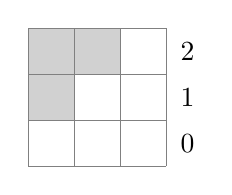
\begin{tikzpicture}[x=.23in,y=.23in]\fill[black!18](0,2)rectangle(2,3);\fill[black!18](0,1)rectangle(1,2);\draw[step=1,black!50](0,0)grid(3,3);\node[right]at(3.1,2.5){2};\node[right]at(3.1,1.5){1};\node[right]at(3.1,.5){0};\end{tikzpicture}}
% Generated by generate-extensions.py; one coordinate unit = one small edge.
\newcommand{\ExtensionMatchingBoard}{\draw[gridline] (0.000000000,0.000000000)--(1.000000000,0.000000000)--(0.500000000,0.866025404)--cycle;\node[font=\small] at (0.500000000,0.288675135) {A};\draw[gridline] (1.000000000,0.000000000)--(2.000000000,0.000000000)--(1.500000000,0.866025404)--cycle;\node[font=\small] at (1.500000000,0.288675135) {B};\draw[gridline] (0.500000000,0.866025404)--(1.500000000,0.866025404)--(1.000000000,1.732050808)--cycle;\node[font=\small] at (1.000000000,1.154700538) {C};\draw[gridline] (1.000000000,1.732050808)--(2.000000000,1.732050808)--(1.500000000,2.598076211)--cycle;\node[font=\small] at (1.500000000,2.020725942) {D};\draw[gridline] (2.000000000,1.732050808)--(3.000000000,1.732050808)--(2.500000000,2.598076211)--cycle;\node[font=\small] at (2.500000000,2.020725942) {E};\draw[gridline] (2.500000000,2.598076211)--(3.500000000,2.598076211)--(3.000000000,3.464101615)--cycle;\node[font=\small] at (3.000000000,2.886751346) {F};\draw[gridline] (3.000000000,1.732050808)--(4.000000000,1.732050808)--(3.500000000,2.598076211)--cycle;\node[font=\small] at (3.500000000,2.020725942) {G};\draw[gridline] (1.000000000,0.000000000)--(1.500000000,0.866025404)--(0.500000000,0.866025404)--cycle;\node[font=\small] at (1.000000000,0.577350269) {H};\draw[gridline] (0.500000000,0.866025404)--(1.000000000,1.732050808)--(0.000000000,1.732050808)--cycle;\node[font=\small] at (0.500000000,1.443375673) {I};\draw[gridline] (1.500000000,0.866025404)--(2.000000000,1.732050808)--(1.000000000,1.732050808)--cycle;\node[font=\small] at (1.500000000,1.443375673) {J};\draw[gridline] (1.000000000,1.732050808)--(1.500000000,2.598076211)--(0.500000000,2.598076211)--cycle;\node[font=\small] at (1.000000000,2.309401077) {K};\draw[gridline] (2.000000000,1.732050808)--(2.500000000,2.598076211)--(1.500000000,2.598076211)--cycle;\node[font=\small] at (2.000000000,2.309401077) {L};\draw[gridline] (2.500000000,0.866025404)--(3.000000000,1.732050808)--(2.000000000,1.732050808)--cycle;\node[font=\small] at (2.500000000,1.443375673) {M};\draw[gridline] (3.000000000,1.732050808)--(3.500000000,2.598076211)--(2.500000000,2.598076211)--cycle;\node[font=\small] at (3.000000000,2.309401077) {N};\draw[outline] (0.000000000,1.732050808)--(1.000000000,1.732050808)--(0.500000000,2.598076211)--(1.500000000,2.598076211)--(2.500000000,2.598076211)--(3.000000000,3.464101615)--(3.500000000,2.598076211)--(4.000000000,1.732050808)--(3.000000000,1.732050808)--(2.500000000,0.866025404)--(2.000000000,1.732050808)--(1.500000000,0.866025404)--(2.000000000,0.000000000)--(1.000000000,0.000000000)--(0.000000000,0.000000000)--(0.500000000,0.866025404)--cycle;}
\newcommand{\ExtensionMatchingSolution}{\draw[tile,fill=white] (0.000000000,0.000000000)--(1.000000000,0.000000000)--(1.500000000,0.866025404)--(0.500000000,0.866025404)--cycle;\node[font=\small] at (0.750000000,0.433012702) {A+H};\draw[tile,fill=white] (0.500000000,0.866025404)--(1.500000000,0.866025404)--(1.000000000,1.732050808)--(0.000000000,1.732050808)--cycle;\node[font=\small] at (0.750000000,1.299038106) {C+I};\draw[tile,fill=white] (1.000000000,1.732050808)--(2.000000000,1.732050808)--(1.500000000,2.598076211)--(0.500000000,2.598076211)--cycle;\node[font=\small] at (1.250000000,2.165063509) {D+K};\draw[tile,fill=white] (2.500000000,0.866025404)--(3.000000000,1.732050808)--(2.500000000,2.598076211)--(2.000000000,1.732050808)--cycle;\node[font=\small] at (2.500000000,1.732050808) {E+M};\draw[tile,fill=white] (3.000000000,1.732050808)--(3.500000000,2.598076211)--(3.000000000,3.464101615)--(2.500000000,2.598076211)--cycle;\node[font=\small] at (3.000000000,2.598076211) {F+N};\draw[tile,fill=black!15] (1.000000000,0.000000000)--(2.000000000,0.000000000)--(1.500000000,0.866025404)--cycle;\node[font=\small] at (1.500000000,0.288675135) {B};\draw[tile,fill=black!15] (3.000000000,1.732050808)--(4.000000000,1.732050808)--(3.500000000,2.598076211)--cycle;\node[font=\small] at (3.500000000,2.020725942) {G};\draw[tile,fill=black!15] (1.500000000,0.866025404)--(2.000000000,1.732050808)--(1.000000000,1.732050808)--cycle;\node[font=\small] at (1.500000000,1.443375673) {J};\draw[tile,fill=black!15] (2.000000000,1.732050808)--(2.500000000,2.598076211)--(1.500000000,2.598076211)--cycle;\node[font=\small] at (2.000000000,2.309401077) {L};\draw[outline] (0.000000000,1.732050808)--(1.000000000,1.732050808)--(0.500000000,2.598076211)--(1.500000000,2.598076211)--(2.500000000,2.598076211)--(3.000000000,3.464101615)--(3.500000000,2.598076211)--(4.000000000,1.732050808)--(3.000000000,1.732050808)--(2.500000000,0.866025404)--(2.000000000,1.732050808)--(1.500000000,0.866025404)--(2.000000000,0.000000000)--(1.000000000,0.000000000)--(0.000000000,0.000000000)--(0.500000000,0.866025404)--cycle;}
\newcommand{\ExtensionLargeBoard}{\draw[gridline] (-1.500000000,2.598076211)--(-1.000000000,1.732050808)--(-0.500000000,2.598076211)--cycle;\draw[gridline] (-1.500000000,2.598076211)--(-1.000000000,3.464101615)--(-0.500000000,2.598076211)--cycle;\draw[gridline] (-1.000000000,3.464101615)--(-0.500000000,2.598076211)--(0.000000000,3.464101615)--cycle;\draw[gridline] (-1.000000000,3.464101615)--(-0.500000000,4.330127019)--(0.000000000,3.464101615)--cycle;\draw[gridline] (-0.500000000,4.330127019)--(0.000000000,3.464101615)--(0.500000000,4.330127019)--cycle;\draw[gridline] (-0.500000000,4.330127019)--(0.000000000,5.196152423)--(0.500000000,4.330127019)--cycle;\draw[gridline] (0.000000000,5.196152423)--(0.500000000,4.330127019)--(1.000000000,5.196152423)--cycle;\draw[gridline] (-1.000000000,1.732050808)--(-0.500000000,0.866025404)--(0.000000000,1.732050808)--cycle;\draw[gridline] (-1.000000000,1.732050808)--(-0.500000000,2.598076211)--(0.000000000,1.732050808)--cycle;\draw[gridline] (-0.500000000,2.598076211)--(0.000000000,1.732050808)--(0.500000000,2.598076211)--cycle;\draw[gridline] (-0.500000000,2.598076211)--(0.000000000,3.464101615)--(0.500000000,2.598076211)--cycle;\draw[gridline] (0.000000000,3.464101615)--(0.500000000,2.598076211)--(1.000000000,3.464101615)--cycle;\draw[gridline] (0.000000000,3.464101615)--(0.500000000,4.330127019)--(1.000000000,3.464101615)--cycle;\draw[gridline] (0.500000000,4.330127019)--(1.000000000,3.464101615)--(1.500000000,4.330127019)--cycle;\draw[gridline] (0.500000000,4.330127019)--(1.000000000,5.196152423)--(1.500000000,4.330127019)--cycle;\draw[gridline] (-0.500000000,0.866025404)--(0.000000000,0.000000000)--(0.500000000,0.866025404)--cycle;\draw[gridline] (-0.500000000,0.866025404)--(0.000000000,1.732050808)--(0.500000000,0.866025404)--cycle;\draw[gridline] (0.000000000,1.732050808)--(0.500000000,0.866025404)--(1.000000000,1.732050808)--cycle;\draw[gridline] (0.000000000,1.732050808)--(0.500000000,2.598076211)--(1.000000000,1.732050808)--cycle;\draw[gridline] (0.500000000,2.598076211)--(1.000000000,1.732050808)--(1.500000000,2.598076211)--cycle;\draw[gridline] (0.500000000,2.598076211)--(1.000000000,3.464101615)--(1.500000000,2.598076211)--cycle;\draw[gridline] (1.000000000,3.464101615)--(1.500000000,2.598076211)--(2.000000000,3.464101615)--cycle;\draw[gridline] (1.000000000,3.464101615)--(1.500000000,4.330127019)--(2.000000000,3.464101615)--cycle;\draw[gridline] (0.000000000,0.000000000)--(0.500000000,0.866025404)--(1.000000000,0.000000000)--cycle;\draw[gridline] (0.500000000,0.866025404)--(1.000000000,0.000000000)--(1.500000000,0.866025404)--cycle;\draw[gridline] (0.500000000,0.866025404)--(1.000000000,1.732050808)--(1.500000000,0.866025404)--cycle;\draw[gridline] (1.000000000,1.732050808)--(1.500000000,0.866025404)--(2.000000000,1.732050808)--cycle;\draw[gridline] (1.000000000,1.732050808)--(1.500000000,2.598076211)--(2.000000000,1.732050808)--cycle;\draw[gridline] (1.500000000,2.598076211)--(2.000000000,1.732050808)--(2.500000000,2.598076211)--cycle;\draw[gridline] (1.500000000,2.598076211)--(2.000000000,3.464101615)--(2.500000000,2.598076211)--cycle;\draw[outline] (0.000000000,0.000000000)--(1.000000000,0.000000000)--(2.500000000,2.598076211)--(1.000000000,5.196152423)--(0.000000000,5.196152423)--(-1.500000000,2.598076211)--cycle;\draw[line width=2pt] (0,0)--(1,0);}
\newcommand{\ExtensionTilingStart}{\draw[tile] (-1.000000000,1.732050808)--(-0.500000000,2.598076211)--(-1.000000000,3.464101615)--(-1.500000000,2.598076211)--cycle;\draw[tile] (-0.500000000,2.598076211)--(0.000000000,3.464101615)--(-0.500000000,4.330127019)--(-1.000000000,3.464101615)--cycle;\draw[tile] (0.000000000,3.464101615)--(0.500000000,4.330127019)--(0.000000000,5.196152423)--(-0.500000000,4.330127019)--cycle;\draw[tile] (0.500000000,4.330127019)--(1.500000000,4.330127019)--(1.000000000,5.196152423)--(0.000000000,5.196152423)--cycle;\draw[tile] (-0.500000000,0.866025404)--(0.000000000,1.732050808)--(-0.500000000,2.598076211)--(-1.000000000,1.732050808)--cycle;\draw[tile] (0.000000000,1.732050808)--(0.500000000,2.598076211)--(0.000000000,3.464101615)--(-0.500000000,2.598076211)--cycle;\draw[tile] (0.500000000,2.598076211)--(1.000000000,3.464101615)--(0.500000000,4.330127019)--(0.000000000,3.464101615)--cycle;\draw[tile] (1.000000000,3.464101615)--(2.000000000,3.464101615)--(1.500000000,4.330127019)--(0.500000000,4.330127019)--cycle;\draw[tile] (0.000000000,0.000000000)--(0.500000000,0.866025404)--(0.000000000,1.732050808)--(-0.500000000,0.866025404)--cycle;\draw[tile] (0.500000000,0.866025404)--(1.000000000,1.732050808)--(0.500000000,2.598076211)--(0.000000000,1.732050808)--cycle;\draw[tile] (1.000000000,1.732050808)--(1.500000000,2.598076211)--(1.000000000,3.464101615)--(0.500000000,2.598076211)--cycle;\draw[tile] (1.500000000,2.598076211)--(2.500000000,2.598076211)--(2.000000000,3.464101615)--(1.000000000,3.464101615)--cycle;\draw[tile] (0.000000000,0.000000000)--(1.000000000,0.000000000)--(1.500000000,0.866025404)--(0.500000000,0.866025404)--cycle;\draw[tile] (0.500000000,0.866025404)--(1.500000000,0.866025404)--(2.000000000,1.732050808)--(1.000000000,1.732050808)--cycle;\draw[tile] (1.000000000,1.732050808)--(2.000000000,1.732050808)--(2.500000000,2.598076211)--(1.500000000,2.598076211)--cycle;\draw[line width=2pt] (0,0)--(1,0);}
\newcommand{\ExtensionPathStart}{\draw[-{Stealth[length=4pt]},line width=1.2pt,dashed] (0.500000000,0.000000000)--(1.000000000,0.866025404);\draw[-{Stealth[length=4pt]},line width=1.2pt,dashed] (1.000000000,0.866025404)--(1.500000000,1.732050808);\draw[-{Stealth[length=4pt]},line width=1.2pt,dashed] (1.500000000,1.732050808)--(2.000000000,2.598076211);\draw[-{Stealth[length=4pt]},line width=1.2pt,dashed] (2.000000000,2.598076211)--(1.500000000,3.464101615);\draw[-{Stealth[length=4pt]},line width=1.2pt,dashed] (1.500000000,3.464101615)--(1.000000000,4.330127019);\draw[-{Stealth[length=4pt]},line width=1.2pt,dashed] (1.000000000,4.330127019)--(0.500000000,5.196152423);}
\newcommand{\ExtensionRouteTableBlank}{\begingroup\renewcommand{\arraystretch}{1.14}\begin{tabular}{c|c@{\hspace{.65in}}c|c}\textbf{Record}&\textbf{Routes}&\textbf{Record}&\textbf{Routes}\\\hline $(0,0,0)$&1&$(2,2,1)$&\rule{.50in}{.35pt}\\$(1,0,0)$&1&$(3,1,1)$&\rule{.50in}{.35pt}\\$(1,1,0)$&\rule{.50in}{.35pt}&$(3,2,0)$&\rule{.50in}{.35pt}\\$(2,0,0)$&\rule{.50in}{.35pt}&$(2,2,2)$&\rule{.50in}{.35pt}\\$(1,1,1)$&\rule{.50in}{.35pt}&$(3,2,1)$&\rule{.50in}{.35pt}\\$(2,1,0)$&2&$(3,3,0)$&\rule{.50in}{.35pt}\\$(3,0,0)$&\rule{.50in}{.35pt}&$(3,2,2)$&\rule{.50in}{.35pt}\\$(2,1,1)$&\rule{.50in}{.35pt}&$(3,3,1)$&\rule{.50in}{.35pt}\\$(2,2,0)$&\rule{.50in}{.35pt}&$(3,3,2)$&\rule{.50in}{.35pt}\\$(3,1,0)$&\rule{.50in}{.35pt}&$(3,3,3)$&\rule{.50in}{.35pt}\\\end{tabular}\endgroup}
\newcommand{\ExtensionRouteTableAnswers}{\begingroup\renewcommand{\arraystretch}{1.14}\begin{tabular}{c|c@{\hspace{.65in}}c|c}\textbf{Record}&\textbf{Routes}&\textbf{Record}&\textbf{Routes}\\\hline $(0,0,0)$&1&$(2,2,1)$&5\\$(1,0,0)$&1&$(3,1,1)$&6\\$(1,1,0)$&1&$(3,2,0)$&5\\$(2,0,0)$&1&$(2,2,2)$&5\\$(1,1,1)$&1&$(3,2,1)$&16\\$(2,1,0)$&2&$(3,3,0)$&5\\$(3,0,0)$&1&$(3,2,2)$&21\\$(2,1,1)$&3&$(3,3,1)$&21\\$(2,2,0)$&2&$(3,3,2)$&42\\$(3,1,0)$&3&$(3,3,3)$&42\\\end{tabular}\endgroup}


\hypersetup{pdftitle={Week 1: Back-pocket extension guide and solutions}}
\begin{document}
\ExtensionTitle{FACILITATOR}{Choose one deeper question}
\RuleBox{These are optional extensions at roughly a \textbf{grades 6--7 reasoning level}. Offer them by readiness, including to a younger child. Each is a separate investigation; the packet is not an extra checklist to finish.}
\Subhead{Which page to pull out}
\renewcommand{\arraystretch}{1.10}
\begin{tabularx}{\linewidth}{@{}>{\raggedright\arraybackslash}p{.8in}>{\raggedright\arraybackslash}X >{\raggedright\arraybackslash}p{1.9in}@{}}
\textbf{Student page}&\textbf{Offer when the child asks\ldots}&\textbf{Prerequisites}\\\hline
1 / X1&``Equal up/down counts should be enough, shouldn't they?''&Pair cells; explain an obstruction.\\
2 + 5 / X2&``Can we predict the distance without drawing the whole graph?''&Read a ribbon; count positions; argue a lower bound.\\
3 / X3&``How many different best routes are there?''&Know the nine-move bound; organized addition; track a three-number record.\\
4 / X4&``If we flip randomly, is every tiling equally likely?''&Read a graph; equal chances; halves and thirds for the proof.\\
\end{tabularx}
\Subhead{Preparation and timing}
Print the student packet single-sided at Actual Size. Mats use the existing nominal one-inch small edge. X1 needs \textbf{7 small blues and 4 greens}; seven blues lets the child attempt a complete filling. X2 needs \textbf{15 small blues} and the large mat, or simply six paper slips: three R and three L. X3 uses those slips and a pencil. X4 needs one counter, a die, and four identical folded number slips. Purple is optional for X1. Set larger pieces aside.

These are alternatives; prepare only the chosen kit. Exchange the original eight-blue board for the fifteen-blue board by adding seven 1\(\times\) blues from the Upscale sets. If the print scale does not match, trace a physical filling or change \texttt{\textbackslash blockside} and rebuild. The 1,3,3,1,3,3 board is not a large regular hexagon.

Allow roughly \textbf{10--20 minutes for X1}, \textbf{15--30 for X2}, \textbf{20--30 for X3}, or \textbf{15--25 for X4's experiment and discussion}. These are flexible planning estimates. Any one may last longer. For only five spare minutes, ask for one obstruction, one pair of words, or a prediction about the random walk; save the rest.
\Subhead{How to launch and when to stop}
Let the child try the first question with objects before giving a hint. Ask for a construction \emph{and} a reason where optimality is claimed. A clear explanation of one surprising example is a useful stopping point. Do not require the general formula or expected-return calculation.

The page references and IDs X1--X4 let you record exactly what was encountered. Keep unused questions available for future sessions. The back-pocket format is supported by \emph{Math Circle by the Bay}, preface pp. ix--x: the authors describe keeping challenging problems ready, using manipulatives, revisiting explanations, and changing depth across ages. These particular tasks and timing estimates are our adaptations.
\Subhead{The mathematical continuations}
X1 leads to Hall's matching condition; X2 to lattice-path encodings and distances in tiling spaces; X3 to recurrence relations, order ideals, and standard Young tableaux; X4 to stationary distributions and return times. Sources and independent verification are recorded in \texttt{plans/week-01-extensions.md}.
\newpage
\ExtensionTitle{X1 / SOLUTION}{A local shortage beats equal totals}
\Subhead{The answer is five blues and four greens}
The board has seven up cells A--G and seven down cells H--N. Yet A and B can pair only with H; F and G can pair only with N. Among \(S=\{A,B,F,G\}\), four up cells compete for just two down partners. At least two of those up cells must remain uncovered by blues.

Every blue removes one up and one down cell. Because the starting counts are equal, the uncovered counts remain equal. At least two uncovered ups therefore force at least two uncovered downs: \textbf{at least four greens}.
\begin{center}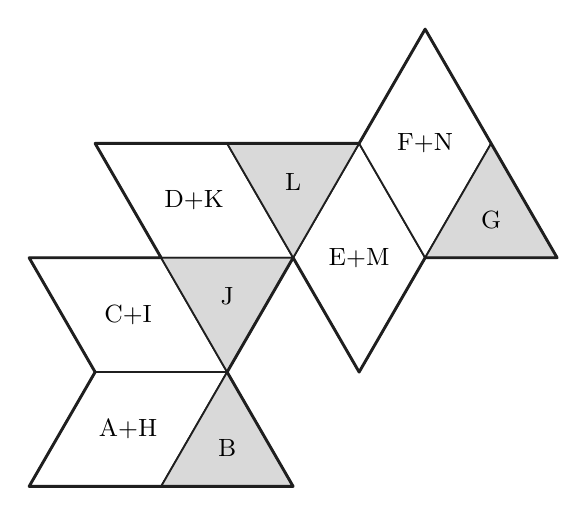
\begin{tikzpicture}[x=.66in,y=.66in]\ExtensionMatchingSolution\end{tikzpicture}\end{center}
The construction attains the bound. Use blues \textbf{A+H, C+I, D+K, E+M, F+N}; put greens at \textbf{B, G, J, L}. All pairs share full sides. Thus four greens is the exact minimum, not merely a lower bound.
\Subhead{Hints, one at a time}
First ask, ``Which cells have only one possible partner?'' Then, ``Can two of them demand the same partner?'' Finally, ``If two ups stay uncovered, what does that force about downs?'' Let the child mark cells and test the partners with a blue.
\Subhead{A useful general statement}
In a board with equal up/down counts, suppose a group of \(k\) up cells has only \(s\) distinct possible down partners, with \(k>s\). At least \(k-s\) up cells are unmatched; balance forces the same number of unmatched downs. Hence there are at least \(2(k-s)\) gaps. This proves a lower bound; it does not by itself construct a packing attaining it.

Adding purple cannot improve the green count: replace each purple by two blues. Any alleged improvement would give a forbidden blue packing with exactly the same gaps. The argument assumes whole printed cells and the specified shapes; pink does not obey that premise.

\textbf{Further challenge:} Design a different connected balanced board with a provable shortage. Specify the competing group, count all its neighbors, and exhibit a best packing. Avoid simply judging a failed experiment to be impossible.
\newpage
\ExtensionTitle{X2 / SOLUTION}{Count words; measure movement}
\Subhead{Twenty tilings and a nine-flip distance}
\textbf{For returners:} Lowell Handout 5, problems 5.5--5.6, counts orders of three cookies of each kind and paths with three east/three north steps. If recognized, reuse that count and move to tiling distances or X3's route counting; do not require a new list of twenty words.

The large board has 30 unit triangles and uses 15 blues. Every ribbon has three R steps and three L steps. Choose the three positions of the L's among six: \(\binom63=20\). Equivalently, there are \(6\cdot5\cdot4\) ordered choices, and each unlabelled choice is counted \(3\cdot2\cdot1\) times. A systematic list works without that notation.

Why words count tilings: there is only one ribbon, since every rhombus with horizontal sides can be followed downward to the sole horizontal bottom edge. The other rhombi all have the third orientation, whose partners are forced. Conversely every three-R/three-L path fits between the extreme paths; the regions on its two sides fill with that third orientation. The supplied geometry independently checks all twenty fillings.

From RRRLLL to LLLRRR each of the three L's must cross each of the three R's, for \(3\cdot3=9\) crossings. One flip makes just one crossing. Repeatedly swapping RL to LR attains nine, proving optimality.
\Subhead{Equal scores can hide distance}
Both \Word{LRRRLL} and \Word{RRLLLR} have score 3, but their distance is \textbf{4}:
\begin{center}\small\Word{LRRRLL}\(\to\)\Word{RLRRLL}\(\to\)\Word{RRLRLL}\(\to\)\Word{RRLLRL}\(\to\)\Word{RRLLLR}.\end{center}
The L positions, from left to right, change from \((1,5,6)\) to \((3,4,5)\). They must move a total of \(2+1+1=4\) places. Each move shifts just one L by one place. This proves no shorter route exists. The difference of scores is a useful lower bound, but it can lose information when some L's need to go left and others right.
\Subhead{The general distance formula}
For two words with the same numbers of R's and L's, number the L's from left to right. If their initial and target positions are \(p_i\) and \(q_i\), the distance is
\[d=\sum_i |p_i-q_i|.\]
The sum is a lower bound because every move shifts one L by one. It is attainable: if an L needs to go left but another L blocks it, follow that adjacent chain leftward. Every blocking L also needs to go left, since the target positions are strictly increasing. The leftmost one has an R to its left and can move one step toward its target. The rightward case is the mirror image. Repeat; each move decreases the sum by one until it is zero.

\textbf{Hints:} Label the L slips without changing their order. Mark their target positions. Ask which L can move toward its target now. For unequal numbers, a word with \(a\) R's and \(b\) L's has \(\binom{a+b}{a}\) possible orders and extreme distance \(ab\); the same ribbon argument applies to the corresponding 1,a,b,1,a,b hexagon.
\newpage
\ExtensionTitle{X3 / SOLUTION}{Forty-two shortest routes}
\Subhead{Why the small record is enough}
On a shortest extreme-to-extreme route, an L only moves left across an R. Let \(x_i\) count the R's crossed by the \(i\)-th L, with L's numbered in their original left-to-right order. They cannot cross one another, so \(3\ge x_1\ge x_2\ge x_3\ge0\). Every legal record determines one word; increasing one coordinate by one while preserving the inequalities is one legal shortest-route move.

The shaded-square model is a left-justified collection of rows. A route adds its nine squares in an allowed order. This is a bijection between shortest word routes and square-adding histories, not just a resemblance between two counting puzzles.
\Subhead{Add the counts at all possible previous records}
There is one empty history at \((0,0,0)\). For every other record, subtract one from a positive coordinate in every way that leaves a valid record; add those counts. Every route has exactly one last step and therefore exactly one previous record. The cases are exhaustive and disjoint.
\begin{center}\ExtensionRouteTableAnswers\end{center}
Thus there are \textbf{42 shortest routes}, although there are only \textbf{20 tilings}. A route is a sequence through states; counting states and counting routes are different questions.
\Subhead{Hints and the next rectangle}
First demonstrate how \((2,1,0)\) comes from \((1,1,0)\) or \((2,0,0)\). If the table feels abstract, shade squares on a \(3\times3\) grid and label the squares by the order added. Read those labels back as a sequence of L moves.

For two R's and four L's, records obey \(2\ge x_1\ge x_2\ge x_3\ge x_4\ge0\). The same recurrence gives \textbf{14 shortest routes}, of length eight; the number of words is \(\binom62=15\). Transposing the four-by-two shaded rectangle gives the equivalent two-row picture.

\textbf{Adult continuation:} Label each added square 1 through 9. Labels increase along rows and columns, producing a standard Young tableau of square shape. Counting such objects leads to the hook-length formula; the recurrence already supplies a complete proof for this small case without invoking that theorem.
\newpage
\ExtensionTitle{X4 / SOLUTION}{Two rules, two long-run answers}
\Subhead{Rule 1: choose uniformly among legal neighbors}
The degrees of A--F are \(1,3,2,2,3,1\). Starting the sharing model with one unit at every node does not preserve equal amounts: after one simultaneous share, A--F receive
\[(1/3,\ 2,\ 2/3,\ 2/3,\ 2,\ 1/3).\]
Instead put \(1,3,2,2,3,1\) units on the nodes. Each node sends exactly one unit along each incident edge and receives one from each neighbor, so its amount is unchanged. Dividing by the total 12 gives stable proportions
\[\pi=(1,3,2,2,3,1)/12.\]
The walk is connected, so these are its long-run visit frequencies: B and E are visited three times as often as A and F. Thirty turns need not resemble these proportions closely. The sharing argument verifies stationarity; the theorem connecting it with long-run averages is an adult continuation.

\textbf{Do not claim ordinary time-step convergence here.} Rule 1 alternates the two parity groups, so its one-time distribution oscillates. Long-run visit frequencies still have the stated limits. A short tally is evidence for a conjecture, not a proof.
\Subhead{Rule 3: choose a fixed label; stay on a failed attempt}
Each edge has chance \(1/4\) in both directions. Node \(v\) stays with probability \(1-\deg(v)/4\). From equal starting amounts, the incoming total is \(\deg(v)/4+1-\deg(v)/4=1\). Thus \textbf{all six nodes have long-run frequency \(1/6\)}. Every node has a stay option, which also removes the parity oscillation. Replacing and remixing the slip after \emph{every} draw is essential.

The labels represent the four possible flip centers on the original small board. X4 can be explored independently on the graph; probabilities are not needed for X1--X3.
\Subhead{Optional return-time answer}
For a finite connected random walk with stationary probabilities \(\pi\), the mean first positive return to a node is \(1/\pi\) at that node. Rule 1 therefore has return means \(12,4,6,6,4,12\), and rule 3 has mean \textbf{6 turns at every node}. A stay at A on the first turn counts; discarding stays changes the experiment.

To derive 12 directly, let \(b,c,e,f\) be mean times to \emph{hit} A from B, C/D, E, F. First-step equations are
\[b=1+2c/3,\quad c=1+(b+e)/2,\quad e=1+(2c+f)/3,\quad f=1+e.\]
They give \((b,c,e,f)=(11,15,17,18)\). A first moves to B, so its return mean is \(1+11=12\). Algebra is optional; stable proportions alone make a substantial extension.

\textbf{Source:} Levin--Peres, \emph{Markov Chains and Mixing Times}, 2nd ed., Example 1.12 and Propositions 1.19--1.20 (printed pp. 9--13); Theorem C.1 (pp. 390--391) for long-run averages. \href{https://pages.uoregon.edu/dlevin/MARKOV/mcmt2e.pdf}{Author-hosted text}. The source notes link Hall's theorem and tiling research.
\end{document}
